%Stil på uppsats
\documentclass[12pt]{article}
\usepackage[utf8]{inputenc}
\usepackage[swedish]{babel}
\usepackage{verbatim}
\renewcommand{\baselinestretch}{1.2}
\renewcommand{\arraystretch}{1.5}

%Skippa indrag av brödtext
\usepackage{parskip}

%Bilder sida vid sida
\usepackage{subfig}

% Formattera text
\usepackage[text={13cm,22cm}]{geometry}

\usepackage{tabularx} %Linea tables med text
\usepackage{booktabs}
\usepackage{floatrow}
\floatsetup[table]{capposition=top}
\usepackage{amsmath}
\usepackage{upgreek}
\usepackage{graphicx}
\graphicspath{{./images/}}
\usepackage{textgreek}
\usepackage{sectsty}
\sectionfont{\large}
\subsectionfont{\small}

\usepackage{afterpage}
\usepackage{sectsty}
\usepackage{caption}
\usepackage{url}
\usepackage{hyperref}
\usepackage{array}
\usepackage{multirow}

% Bibliography
\usepackage[style=authoryear,sorting=nty]{biblatex} %Imports biblatex package
\addbibresource{references.bib} %Import the bibliography file

\usepackage[referable]{threeparttablex}
\usepackage{booktabs}
\usepackage{lipsum}

\usepackage[export]{adjustbox} %För titelsida


\begin{document}
\begin{titlepage}
\thispagestyle{empty}
	\begin{figure}[ht]
	   \minipage{0.75\textwidth}
			\includegraphics[width=7cm]{stat.png}
			
	   \endminipage
	    \minipage{0.32\textwidth}
		 \includegraphics[height = 3.5cm,width=4cm]{SU1.jpg}
			
\endminipage
\end{figure}
	
	
\centering
\vspace{5cm}

{\large\bfseries LSTM ARMA-GARCH\par}
	\vspace{0.5cm}
	
{\large\itshape Kandidatuppsats statistik \par}
	\vfill
	
\begin{flushleft}
Författare: Erik \& Erik \\
Handledare: Ulf Högnäs\\
ST312G Kandidatuppsats i statistik \\
VT21
\end{flushleft}
\end{titlepage}


%%%%%%%%%%%% ABSTRACT %%%%%%%%%%%%%%%%%
\newpage
\thispagestyle{empty}
\section*{Sammanfattning}
TODO

%%%%%%%%%%%% TABLE OF CONTENTS %%%%%%%%%%%%%%%%%
\newpage
\tableofcontents
\newpage

\begin{comment}
Hej igen!

Här kommer vårat först utkast. Säg gärna till när du tror att du har möjlighet att hunnit läsa igenom det och kan ta ett videomöte.

Det förekommer definitivt slarvel (formalia, ekvationer som har fel namn osv) men vi har inte prioriterat att fixa dessa just nu, utan tar det inför slutinlämningen (det lär ändå hinna ändras)

Två frågor vi vill skicka med är:
- Vad tycker du vi kan utveckla för att ta detta till nästa nivå? Det känns som vi har både tid och plats att göra något extra.
- En idé vi har är att simulera en trading-strategi likt http://cs230.stanford.edu/projects_winter_2020/reports/32066186.pdf, för att se vilken av modellerna som hade varit bäst att tradea med. Det ger också mer relaterbara resultat eftersom vi kan sätta ett pengavärde på hur bra modellerna presterar. Vad tror du om det?

Ser fram emot din feedback!

Allt gott,

Erik & Erik
\end{comment}

%%%%%%%%%%%%%% Förkortningar %%%%%%%%%%%%%%%
\newpage 

\section*{Lista över förkortningar}
\textbf{AIC} - Akaike Information Criterion \par
\textbf{ANN} - Artifical Neural Network \par
\textbf{ARCH} - Autoregressive Conditional Heteroskedasticity \par
\textbf{ARIMA} - Autoregressive Integrated Moving Average \par
\textbf{ARMA} - Autoregressive Moving Average \par 
\textbf{ARMA-GARCH} - Autoregressive Moving Average - Generalized Autoregressive Conditional Heteroskedasticity \par 
\textbf{BIC} - Schwarz Bayesian Information Criterion \par
\textbf{EMH} - Efficient Market Hypothesis (sv: Effektiva marknadshypotesen) \par
\textbf{GARCH} - Generalized Autoregressive Conditional Heteroskedasticity \par
\textbf{LSTM} - Long Short-Term Memory \par
\textbf{MAPE} - Mean Absolute Percentage Error \par
\textbf{OMXSSC} - OMX Stockholm Small Cap \par
\textbf{RMSE} - Root-Mean-Square Error \par
\textbf{RNN} - Recurrent Neural Network \par

\newpage
%%%%%%%%%%%%%% INLEDNING %%%%%%%%%%%%%%%
\clearpage
\setcounter{page}{1}

\section{Inledning}
Att förutspå aktiemarknaden sysselsätter miljontals människor världen över. Målet är att förutspå prisförändringar och på så vis tjäna pengar. Med tanke på aktiemarknadnaden volatititet är det såklart komplicerat. Det finns dock såväl statistisk- samt maskininlärningsmodeller att tillgå för att underlätta. Denna uppsats jämför två olika typer av sådana vanligt förekommande modeller. \par
Jämförelsen mellan de olika modellerna kan ses som en jämförelse mellan det traditionella och det moderna. Maskininlärning och AI är väl omskrivet och anses av många vara framtiden. Populariteten har också gjort att det blivit allt enklare att applicera modeller, Microsoft har exempelvis en tjänst där det går att träna maskininlärningsmodeller utan att ens kunna programmera \parencite{lobe}. Statistisk, å andra sidan, kan uppfattas som mer förlegat, inte lika modernt. Det bör dock noteras att många maskininlärningsmodeller baseras på välkända statistiska koncept såsom regression. En jämförelse mellan söktrender på Google (se Figur 1) visar hur relativa sökningar på termen 'machine learning' kraftigt ökat under 2010-talet, medan 'statistics' snarare minskat \parencite{trends_ml, trends_statistic}. 
\begin{figure}[h]
\caption{Jämförelse av relativa mängden sökningar för 'statistics' och 'machine learning' över tid.}
\includegraphics[width=0.7\linewidth]{ml_vs_stat.png}
\centering
\end{figure}
Det är den här jämförelsen, mellan statistikmodellen ARMA-GARCH och maskininlärningsmodellen LSTM, denna uppsats syftar att utföra. Rent konkret söker uppsatsen att besvara frågeställningen: \par 
\emph{Vilken av modellerna LSTM eller ARMA-GARCH genererar mer precisa prediktioner?}. \par
Detta kommer att göras genom att anpassa respektive model till ett dataset över ett småbolagsindex på Stockholmsbörsen och sedan jämföra magnituden av fel modellerna gör när de predicerar utvecklingen på indexet under en dag, en halv börsvecka, en hel börsvecka, en börsmånad och ett börskvartal framåt i tiden. \par 
Upplägget för uppsatsen är som följer: I avsnitt 1.1 presenteras tidigare studier, i 1.2 avgränsningar, i avsnitt 2. presenteras metoden och datamaterialet, i avsnitt 3. presenteras resultatet av analysen och i avsnitt 4. diskuteras resultaten och slutsatserna av studien. \par


%%%%%%%%%%%%%% TIDIGARE STUDIER %%%%%%%%%%%%%%%
\subsection{Relaterad forskning}

Siami-Namini \& Namin (2018) undersöker i en studie huruvida RMSE skiljer sig mellan LSTM och ARIMA på ett flertal världsindex, däribland DJI och Nikkei 225, och finner bevis för att LSTM överträffar ARIMA i förmågan att reducera av prediktionsfel. Qiu, Song och Akagi (2016) finner likt Siami-Namini \& Namin (2018), att ANN med födel kan användas för att prediktera framtida avkastning på Nikkei 225. 

Jeong \& Lee (2019) applicerade en tangentfunkton i ARMA-komponenten och fann bevis för att en modifierad icke-linjär ARMA-GARCH modell med liknande egenskaper som en RNN predikterar framtida avkastningen på S\&P500 bättre än en ordinär ARMA-GARCH med linjära egenskaper. Detta är i linje med Sun, Xiao et al. (2019). Sang, Di Pierro (2018) applicerade LSTM och fann bevis att en trading-strategi baserad på ANN generarar högre avkastning klassisk teknisk analys. 

Gemensamt för de flesta studier utifrån svenska index är att de jämfört djurinlärningsalgoritmer med ARIMA, denna studie berör ARMA-GARCH på ett småbolagsindex med kortare prediktionsperioder och empiriska valideringsmetoder. Det finns ett flertal studier som berör storbolagsindex för ett enskilt land eller ett världsindex. Empiriska studier utifrån svenska index, synnerligen småbolagsindex som är mer volatilt, är mer sällsynt vilket vi i denna studie vill bidra med. 

 
%%%%%%%%%%%%%% AVGRÄNSNINGAR %%%%%%%%%%%%%%%
\subsection{Avgränsningar}
Uppsatsen är begränsad till att enbart beröra small-cap index på Stockholmsbörsen. Slutsatserna av analysen av vilken metod som är bäst går således inte nödvändigtvis att applicera på andra index eller enskilda aktier. Resultatet går inte heller nödvändigtvis att generalisera utanför de valda prediktionsperioderna.

%%%%%%%%%%%%%% TEORI %%%%%%%%%%%%%%%
\section{Finansiell teori}
\subsection{Hypotesen om effektiva marknader (EMH)}
Den effektiva marknadshypotesen, även känd som EMH, är en term som definerades första gången av Harry Roberts (1967) och utvecklades några år senare av Eugene Fama (1970) \parencite{EMHhistory} i artikeln \emph{"Efficent Capital Markets: A Review of Theory and Empirical Work"}. 

EMH är starkt förknippat med slumpvandring s.k. \emph{Random Walk}, som karakteriseras av en prisserie där alla efterföljande prisförändringar är slumpmässiga avvikelser från sin tidigare prisnivå. Om investerare har obehindrad tillgång till information och detta återspeglas direkt i prisnivån kommer morgondagens prisförändringar vara oberoende av dagens prisförändringar \parencite{EMH}. Vidare kan EMH delas upp i tre olika definitioner av marknadseffiktivitet: \emph{Svag form}, \emph{halvsvag form} och \emph{stark form} \parencite{Fama1970}. \emph{Svag form} betyder att framtida priser omöjligt kan predikteras genom att analysera historisk data. \emph{Halvstark form} är en mer restriktiv variant som inkluderas av att all offentlig information redan reflekterats i priserna. \emph{Stark form} som är den mest restriktiva innebär att prisnivån återspeglar all information som finns tillgänglig.

I sin strängaste form säger EMH att det inte går att göra prognoser av spekulativa priser, detta eftersom om framtida prisnivåer gick att prediktera med hjälp av statistiska modeller skulle investerare använda dessa för att konsekvent generera hög avkastning. Detta beteende skulle därmed medföra att marknaden med tiden underställer sig EMH och det skulle vara hopplöst att finna en modell som presterar bättre än en slumpvandring med drift. \parencite{EMHforecast}. EMH i dess strängaste form har dock kritiserats och delvis motbevisats \parencite{basu1977investment, ball1978anomalies}.

% TEORTEISKT RAMVERK
\section{Teoretiskt ramverk}
\subsection{Logaritmerad avkastning}
Vid analys av finansiella tidsserier är logaritmerad avkastning att föredra då det gör den symmetrisk - positiva och negative procentuella ordinarie avkastningar av samma magnitud tar ut varandra. Detta gör den enklare att arbeta med och har fördelaktiga statistiska egenskaper gentemot en prisserie då denna sällan är stationär \parencite{Tsay2010}.

Låt \(P_t\) vara stängningspriset och $R_{t}=\frac{P_{t} - P_{t-1}}{P_t-1}$ vara nettoavkastningen, bruttoavkastningen mellan period $t$ och $t-1$ kan då defineras som

\begin{equation*}
    1+R_{t} = \frac{P_{t}}{P_{t-1}} = P_{t-1}(1+R_{t})
\end{equation*}

Den naturella logaritmen av avkastningen under period $t$ kan då defineras som

\begin{equation*}
    r_{t}=ln(1 + R_{t})=ln\Big(\frac{P_{t}}{P_{t-1}}\Big)=p_{t}-p_{t-1}
\end{equation*}

Eftersom prisnivåer är mer tolkningsbara kan de logaritmerade värdena med fördel transformeras om till prisnivå efter att skattnignar gjorts. Den kumulativa summan av den logaritmerade avkastningen under perioden exponentieras enligt

\begin{equation*}
    \text{Prisnivå} =  exp\Big({\sum\limits_{t=1}^n \theta_{t}} + ln(\phi)\Big)
\end{equation*}

Där  $\theta$ är det predikterade värdet för tidpunkt $t$ och $\phi$ det sista predikterade värdet för träningsdatan. 


%forecasted_price = exp(cumsum(forecast) + log(last_train))




\subsection{Stationäritet}
Stationäritet är centralt vid analys av tidsserier. En väsentlig egenskap hos stationära tidsserier är de inte påverkas av stora temporära förändringar (s.k. chocker) över tid, utan dessa effekter försvinner relativt snabbt. I en icke-stationär tidsserie förblir chocker och påverkar framtida värden på tidsserien. \par
I strikt mening innebär stationäritet att tidsserien uppvisar liknande 'statistikt beteende' över tid. Vanligtvis används dock svag stationäritet, vilket definieras som 1) tidsseriens förväntade värde beror inte på tid, \(E(y_t)=\mu_y\) och 2) autokovariansfunktionen är enbart en funktion av k och inte tid, \(\gamma_y(k) = Cov(y_t, y_{t+k})\) \parencite{montgomery2015forecasting}. För att illustrera stationäritet följer ett exempel på en typiskt stationär och en typiskt icke-stationär tidsserie.

\begin{figure}[H]
\caption{Illustration av stationäritet med simulerad data}
\includegraphics[width=0.9\linewidth]{stationarity.png}
\centering
\end{figure}

\subsubsection{Test för stationäritet}
För att testa stationäritet kan Augmented Dickey-Fuller test användas \parencite{dickey1979distribution}. Nollhypotesen är att en enhetsrot finns, \(\phi=1\) och alltså ingen stationäritet. Alternativhypotsen är att \(\phi<1\). Definiera \(\theta = \phi -1 \) för att kunna testa \(H_0:\theta=0\) i en regression. Låt \(y_t\) vara beroende variabeln, \( \alpha \) en konstant, \( \gamma \) en koefficient, \(e\) är felterm och p antal laggar \parencite{wooldridge2018introductory}. Formeln är som följer:

\begin{equation*}
    \Delta y_t = \alpha + \theta y_{t-1} + \gamma_1\Delta y_{t-1} + ... + \gamma_p\Delta y_{t-p} + e_t
\end{equation*}
\begin{equation}
        = \alpha + \theta y_{t-1} + \sum_{t=1}^{p}\gamma_p \Delta y_{t-p} + e_t
\end{equation}

Om \(\theta\) är skild från noll förkastas alltså nollhypotesen att ingen stationäritet finns.

\subsection{ARMA-GARCH}
Som diskuterades i introduktionen har tidigare studier använt ARIMA för prediktioner. Nackdelen med ARIMA är dock att variansen antas vara konstant vilket visat sig sällan vara sant inom finansiell analys \parencite{montgomery2015forecasting}. För att hantera inkonstant varians (heteroskedasticitet) utvecklades ARCH och GARCH av Engle \parencite*{engle1982autoregressive} respektive Bollerslev \parencite*{bollerslev1986generalized}. Nackdelen är dock att ARCH/GARCH inte fångar systematiska skillnader i medelvärde över tid. Genom att kombinera ARMA och GARCH till en hybridmodel, ARMA-GARCH, går det att fånga systematiska skillnader i medelvärdet av tidsserien över tid med ARMA-komponenten såväl som systematiska skillnader i varians med GARCH-komponenten. Modellen är relativt ny men har snabbt blivit populär inom flera olika områden \parencite{chen2011short}. 
\par Notera att skillnaden mellan ARIMA(p,d,q) och ARMA(p,q) är att den tidigare möjliggör differentiering med parametern d. Uppfylls stationäritet finns dock ingen anledning att differentiera ytterligare och ARIMA(p,0,q) blir då identisk med ARMA(p,q). 
\par Nedan följer formeln för modellen. \(e_t\) är vitt brus (felterm), \(delta\) en konstant, \(\phi_i\) vikter för laggade beroende variabel i AR(p), \(\theta_i\) vikter för laggade feltermen i MA(q), \(z_t\) är oberoende och identiskt fördelade med medelvärde 0 och varians 1, w en konstant, \(\alpha_i\) vikt för ARCH-termen och \(\beta_i\) vikt för GARCH-termen \parencite{bollerslev1986generalized, montgomery2015forecasting}.

\begin{equation}
    y_t = \delta + \sum_{i=1}^{p}\phi_iy_{t-i}  +e_t - \sum_{i=1}^{q}\theta_i e_{t-i} 
\end{equation}
\begin{equation}
    e_t=\sqrt{\sigma_t}*z_t,\quad \sigma^2_t=w + \sum_{i=1}^{q}\alpha_i e^2_{t-i} + \sum_{i=1}^{p}\beta_i \sigma^2_{t-i}
\end{equation}

Förenklat uttryckt modellerar alltså ARMA den beroende variabeln i (2) och GARCH feltermern i (3).

\subsubsection{Test för heteroskedasticitet}
Som tidigare nämnts finns ingen anledning att använda GARCH-komponenter om det inte finns tecken på heteroskedasticitet. För att testa om tidsserien är heteroskedastisk används Lagrange Multiplier test (LM-test). LM-testet utgår från att modellera bästa möjliga AR-modell, sedan ta dess kvadrerade feltermerna \(e_t^2\) och modellera en regression på dessa. Regressionen består av en konstant \(\alpha_0\) och laggade feltermer \(e_{t-i}\) enligt:

\begin{equation}
    e_t^2=\alpha_0+\sum_{i=1}^{p}\alpha_ie_{t-i}^2
\end{equation}

Nollhypotesen är att alla \(\alpha_i\) = 0, vilket tyder på avsaknad av ARCH-komponenter i feltermen (homoskedasticitet). Alternativhypotesen är att sådana komponenter finns (heteroskedasticitet) och därför att det finns belägg för att använda ARCH och/eller GARCH-modeller \parencite{engle1982autoregressive}. \par

\subsubsection{Val av optimal modell}
En statistika behövs för att avgöra vilket antal tidslaggar (p och q) som är optimalt för ARMA-GARCH-modellen. Två vanligt förekommande sådan mått är Akaike Information Criterion (AIC) samt Schwarz Bayesian Information Criterion (BIC). Modellerna bestraffas för att inkludera ytterligare parametrar, vilket alltså gör det perfekt för att hitta optimalt antal laggar (en ytterligare lag mostvarar en ytterligare parameter). Ju lägre värde, desto bättre \parencite{montgomery2015forecasting}. Låt T vara antal observationer, e felterm och p antal parametrar:
\begin{equation}
    AIC = ln\left( \frac{\sum_{t=1}^{T}e^2_t}{T} \right)+\frac{2p}{T}
\end{equation}
\begin{equation}
    BIC = ln\left( \frac{\sum_{t=1}^{T}e^2_t}{T} \right)+\frac{ln(T)p}{T}
\end{equation}


\subsection{Long Short-Term Memory (LSTM)}
Long Short-Term Memory (LSTM) är en typ av upprepat neuralt nätverk (en: recurrent neural networks, RNN). För att förstå LSTM behövs en grundläggande förståelse av neurala nätverk. \par

Ett neuralt nätverk är en struktur av sammankopplade neuroner, inspirerad av biolgiska neurala nätverk. Nätverket består av flertalet olika algoritmer som tillsammans utför beräkningar. Upprepade neurala nätverk (RNN) är neurala nätverk som är särskilt bra på att hantera temporär data. Varje neurons celler har ett 'minne', där all indata behandlas med hjälp av loopar. På så sätt kan de 'komma ihåg' tidigare data. Dock inte särskilt länge, vilket är varför LSTM behövs \parencite{purkait2019hands}. \par
LSTM-nätverk kan behålla information i ett 'långsiktigt minne' (en: \textit{state}), som förs över mellan tidsperioder. En LSTM-cell ser ut som följer:
\begin{figure}[H]
\caption{LSTM-cellens struktur \parencite[lånad från][]{yuan2019nonlinear}}
\includegraphics[width=10cm]{lstm.png}
\centering
\end{figure}

Varje LSTM-cell har tre indata; minnet från tidigare steg \(c_{t-1}\), indatan från tidigare steg \(h_{t-1}\) och den nya indatan \(x_{t}\). De mörkblåa fyrkanterna märker de tre 'grindarna' som finns i LSTM. Först kommer 'forget gate', det är den som gör att LSTM skiljer sig från vanliga RNNs. Detta eftersom 'forget gate' bestämmer huruvida indatan från tidigare steg (\(h_{t-1}\)) ska behållas eller förkastas från state. Beslutet görs baserat på värdet i förra tidsperioden och den nya indatan, genom att ge denna olika vikter mellan 0 och 1 (där 1 är högst vikt). 'Input gate' kontrollerar flödet av information i det befintliga cellminnet. Denna grind bestämmer vilken ny information som ska läggas till i state. I den sista grinden, 'output gate', avgörs vad som ska läggas till i det 'dolda state' (\(h_{t}\)) inför nästa tidsperiod. Sammanfattningsvis tar varje neurons cell emot tre indata och skicka vidare två utdata till nästa cell. Detta itereras sedan över alla datapunkter och efter den sista iterationen omvandlas 'dolda state' till utdata i önskat format. \parencite{purkait2019hands} \par
Väldigt förenklat kan det alltså förklaras som  att för varje tidpunkt i datan (i detta fall priser på small cap index) skickas datan in i LSTM-cellerna, itereras i dessa där det avgörs vad som ska tas med i beräkningarna av nästa datapunkt (t+1), itereras sedan över alla datapunkter och till slut görs prediktioner baserat på modellen. \par
Definiera \(x_t\) som indatavektorn, \(f_t\) som 'forget gates' aktiveringsvektor, \(i_t\) 'input gate' aktiveringsvektor, \(O_t\) 'output gate' aktiveringsvektor, \(h_t\) 'dolda state' vektorn (även kallad utdatavektorn), \(\tilde{c_t}\) cellens indataaktiveringsvektor, \(c_t\) cellens statevektor, \(W, U, b\) vikt- och biasmatriser som modellen lär sig under träning. \(\sigma\) är sigmoidfunktion och tanh hyperbolisk tangentfunktion. Cirklarna representerar elementvis produkt. Nedsänkt i hänvisar till 'input gate', nedsänkt o till 'outpunk gate', nedsänkt f till 'forget gate', c till minnescellen och t till tidpunkt \parencite{purkait2019hands}. 

\begin{equation}f_t = \sigma(W_f x_t + U_f h_{t-1} + b_f)\end{equation}
\begin{equation}i_t = \sigma(W_i x_t + U_i h_{t-1} + b_i)\end{equation}
\begin{equation}o_t = \sigma(W_o x_t + U_o h_{t-1} + b_o)\end{equation}
\begin{equation}\tilde{c}_t = tanh(W_c x_t + U_c h_{t-1} + b_c)\end{equation}
\begin{equation}c_t= f_t \circ c_{t-1} + i_t \circ \tilde{c}_t\end{equation}
\begin{equation}h_t= o_t \circ tanh(c_t)\end{equation}

Sammanfattat styr alltså (7) vad som händer i 'forget gate', (8) 'input gate' och (9) 'output gate'. I (10) kombineras dessa tre ekvationer, i (11) skapas utdatan och den multipliceras sedan med det befintliga 'dolda state' i (12). 


\section{Metod och datamaterial}
I det här avsnittet beskrivs de modeller som används, varför de väljs och hur de utvärderas. En beskrivning över dataset görs också. 

%%%%%%%%%%%%%% DATAMATERIAL %%%%%%%%%%%%%%%
\subsection{Datamaterial}

Data på dagliga stängningspriser är hämtat från Refinitiv Eikon och täcker perioden från 12 februari 2001 till 12 februari 2021. I syfte att prediktera ett svenskt småbolagsindex används data på historiska stängningspriser på OMX Stockholm Small Cap (OMXSSC) som därefter transformeras till logaritmerad avkastning. Alla priser är i SEK. I OMXSSC inkluderas data från totalt 93 svenska småbolag, vilka defineras som bolag med ett börsvärde som understiger 150 miljoner euro \parencite{smabalagsdefinition}. I \emph{Figur 5} syns en tidsserie över stäningspriserna under perioden.

\begin{figure}[H]
\caption{Prisserie över OMXSSC}
\includegraphics[width=\linewidth]{data.png}
\centering
\end{figure}

I Figur -.- syns den logaritmerade avkastningsserien, perioder med hög volatilitet kännetecknas av aggressiva prisförändringar i avkastningsserien under en given period.

\begin{figure}[H]
\caption{Logaritmerade avkastningsserie över perioden}
\includegraphics[width=\linewidth]{logplot.png}
\centering
\end{figure}

Nedan i \emph{Tabell 1} visas deskriptiv statistik tillsammans med de två momenten \emph{skevhet} och \emph{kurtosis}. 

\begin{table}[H]
\caption{Deskprivtiv statistik och moment}
\scalebox{0.61}{
\begin{tabular}{|c|c|c|c|c|c|c|c|c|c|}
\hline
Index & Start & Slut & N & Min. & Medelvärde & Max. & SD & Skevhet & Kurtosis \\ \hline
OMXSSC   & 2002-12-30 & 2021-02-12 & 4564 & -0.087409 & 0.00555 & 0.070059 & 0.000555 & -1.443848 & 12.914934 \\ \hline
\end{tabular}}
\end{table}

Skevhetskoefficienten för avkastningsserien är negativ - fördelningen har en lång negativ svans med större frekvens av negativa avkastningar jämfört med positiva avkastningar. Kurtosiskoefficienten är större än tre och kännetecknas av en tjock svans (En: "\emph{fat tail}") där dagar med onormalt hög avkastning förekommer mer frekvent än hos en normalfördelning.





Prediktioner görs en, tre och fem dagar fram i tiden. För att utvärdera modellerna har avkastningsserien delats in i träningsdata (75\%) och testdata (25\%). Där den första används för att göra prediktioner och den senare för jämförelse. 


\subsection{Tidsseriemodeller}
\subsubsection{ARMA-GARCH}
En förutsättning för att använda ARMA-GARCH är att tidsserien är stationär, därför används Augmented Dickey-Fuller-testet. Genom funktionen \textit{ur.df} (paket: URCA) väljs automatiskt optimalt antal laggar baserat på AIC och sedan utförs testet.
\par En annan förutsättning är att feltermerna av en ARIMA är heteroskedastiska, därför görs LM-testet på bästa möjliga ARIMA-modell (genom funktionen \textit{auto.arima} i R). 
\par Givet att det inte finns belägg för homoskedasticitet väljs sedan bästa möjliga ARMA-GARCH-modell baserat på AIC och BIC. 



\subsubsection{Long Short-Term Memory (LSTM)}
För att skatta en LSTM behöver modellen så kallade hyperparametrar. Dessa hyperparametrar är olika för olika modeller och alla behöver inte specifieras. Tidigare studier hävdar till och med att värdet på hyperparametrarna inte har en väsentlig påverkan på utfallet \parencite{dreyfus2005neural}. Nedan följer de parametrar där det finns andra studier på hur de bör specifieras. Eftersom övriga parametrars specifikation inte ska ha någon väsentlig påverkan har dessa valts utifrån vad som är vanligt förekommande. Antal laggar har valts till lika många som i ARMA-GARCH för jämförbarhetens skull.

Hyperparametrarna med gedigen forskning bakom sig är \emph{loss function, optimizer och epochs}. \par
\emph{Loss function} är ett mått på hur väl modellen presterar på träningsdatan. Förlustfunktionen används som ett mått på modellens fel och detta ska minimeras. MSE (Mean Square Error) rekommenderas för de flesta 'regressionsliknande' modeller, och därför även i detta fall \parencite{purkait2019hands}. \par
\emph{Optimizer} är den typ av algoritm som används för att minimera det ovan beskrivna felet. 'Adam' är en optimeringsalgoritm som visat sig fungera bra för stora dataset och rekommenderas av Purkait \parencite{purkait2019hands}. \par
\emph{Epochs} indikerar antal gånger modellen kommer att itererar genom hela datasetet. Tidigare studier har kommit fram till att valet inte har någon relevant betydelse för hur väl modellen presterar \parencite{siami2018forecasting}. Då Purkait använder fem epoker för LSTM, kommer även denna uppsats använda fem \parencite{purkait2019hands}. \par


%%%%%%%%%%%%%% VALIDERING %%%%%%%%%%%%%%%
\subsection{Valideringsmetoder}
\subsubsection{RMSE}
För att mäta hur mycket de skattade stängningspriserna avviker från de verkliga stäningspriserna används RMSE (Root Mean Square Error), som ett mått på medelvärdet av standardfelen. Den bärande egenskapen hos RMSE är att större prediktionsfel får relativt större vikt då måttet baseras på ett viktat medelvärde enligt

\begin{equation*}
RMSE = \sqrt{\frac{1}{n}\Sigma_{i=1}^{n}   (\hat{\theta_{t}} - \theta_{t}})^2
\end{equation*}

där \emph{n} är det totala antalet observationer, $\theta_{t}$ är den faktiska prisnivån och $\hat{\theta_{t}}$ är den skattade prisnivån under handelsdag \emph{t}. 

\subsubsection{MAPE}
Utöver RMSE används även MAPE (Mean Absolute Percentage Error) som har liknande egenskaper som RMSE men mäter de absoluta avvikelserna relativt nivån hos $\theta$, vilket ger de relativa avvikelserna i procent enligt

\begin{equation*}
    \textit{MAPE}=\frac{1}{n} 
    \sum_{t=1}^{n} \vert \frac{A_{t}-F_{t}}{A_{t}} \vert \times 100
\end{equation*}

där $A_{t}$ är det aktuella stängningspriset under handelsdag $t$, $F_{t}$ är det predikterade stängningspriset och $n$ är antalet anpassade datapunkter som absolutbeloppet divideras med. 

\subsubsection{Precision, känslighet och F-värde}
För att mäta hur väl modellerna predikterar en stigande respektive fallande prisnivå används en sammanblandningsmatris som registrerar antal korrekta och inkorrekta klassifikationer \parencite{ModelValidation}. I Tabell 1 syns en sammanblandningsmatris för den binära klassifikationen. 

\begin{table}[H]
\caption{Binär klassifikation}
\scalebox{0.95}{
\begin{tabular}{l|l|c|c|c}
\multicolumn{2}{c}{}&\multicolumn{2}{c}{\textbf{Prediktion}}&\\
\cline{3-4}
\multicolumn{2}{c|}{}&Stigande&Fallande&\multicolumn{1}{c}{}\\
\cline{2-4}
\multirow{2}{*}{\rotatebox{90}{\textbf{Aktuell}}}& Stigande & \emph{Sann stigande (SS)} & \emph{Falskt fallande (FF)} &\\
\cline{2-4}
& Fallande & \emph{Falskt stigande (FS)} & \emph{Sann fallande (SF)} & \\
\cline{2-4}
\end{tabular}}
\end{table}

Tre vanligt förekommande mått relaterade till sammanblandningsmatrisen är precision, känslighet och F-värde (KÄLLA?). Måtten ger tillsammans en bra överblick över hur ackurat modellen är.

\par Precision ger svar på frågan 'Vilken andel av predikterade positiva stiganden är korrekta?'. Den mäts alltså av andelen korrekt skattade stigande prisnivåer enligt:
\begin{equation}
    \textit{Precision} = \frac{\sum(SS)}{\sum(SS)+\sum(FS)} 
\end{equation}

Känslighet ger svar på frågan 'Vilken andel av faktiska uppgångar var korrekt identifierade?'. Skillnaden mot precision kan beskrivas som att precision mäter 'givet att prediktionen var ökat värdet, gick värdet upp?' medan känslighet mäter 'givet att värdet har ökat, var prediktionen korrekt?'. Känslighet mäts genom att dividera antalet korrekt skattade stigande prediktioner med det totala antalet stigande prisnivåer enligt:

\begin{equation}
    \textit{Känslighet} = \frac{\sum(SS)}{\sum(SS)+\sum(FF)}
\end{equation}

F-värde är en kombination av ovan nämnda mått och mäter ett tests ackuratess. Utifrån ekvation (2) och (3) kan F-värdet härledas enligt:

\begin{equation}
    \textit{F} = \frac{(\beta^2+1) \times \textit{Precision} \times \textit{Känslighet}}{\beta^2 \times \textit{Precision} + \textit{Känslighet}}
\end{equation}

Precision och känslighet viktas lika, då det inte finns någon bra anledning att göra annat. För att vikta måtten lika används $\beta=1$ \parencite{ModelValidation}, enligt

\begin{equation}
    \textit{F1} = 2 \times \frac{\textit{Precision} \times \textit{Känslighet}}{\textit{Precision} + \textit{Känslighet}}
\end{equation}

Där $F1=1$ är det högsta värdet vilket betyder att modellen inte har några felaktiga predikteringar. $F1=0$ är det lägsta värdet och indikerar att samtliga skattningar om framtida prisnivåer utifrån modellen är felaktiga.


\subsubsection{Korsvalidering}
Tidsserien korsvalideras med rullande fönster (en: \textit{k-fold cross-validation}). Det innebär att träning- och testdata flyttas en period framåt från dess ursprungliga startpunkt i n perioder. Vid nästa period inkluderas alltså det första värdet som predicerades mot i det nya träningssetet \parencite{bergmeir2018note}. I denna uppsats kommer 1000 perioder används. Nedan figur förtydligar vad som händer:
\begin{figure}[H]
\caption{Illustration av rullande fönster-korsvalidering med fyra perioder.}
\includegraphics[width=0.9\linewidth]{cross_validation.png}
\centering
\end{figure}
Fördelen med denna typ av korsvalidering är att prediktioner görs vid 1000 olika punkter istället för att utgå från en enstaka punkt. Att 1000 perioder görs möjliggör även medelvärdesanalys av valideringsmåtten och på så sätt en statistisk jämförelse mellan de olika måtten. För att jämföra medelvärdena av måtten kommer z-test användas. Det är motiverat att använda z-test eftersom antal observationer är väldigt många (1000). 
\par Låt \(\Bar{x}_i, i=\{1,2\}\) vara medelvärdet för variabel i, \(s_i^2\) standardavvikelsen för variabel i och \(n_i\) antal observationer för variabel i. Alternativhypoteserna \(H_1\) beror på om det testas om värdet är högre eller lägre än det andra värdet.

Hypoteserna är:
\begin{equation*}
    H_0: \Bar{x}_1 - \Bar{x}_2 = 0 \Leftrightarrow \Bar{x}_1 = \Bar{x}_2
\end{equation*}
\begin{equation*}
    H_1: \Bar{x}_1 - \Bar{x}_2 < 0 \Leftrightarrow \Bar{x}_1 < \Bar{x}_2
\end{equation*}
\begin{equation}
    H_1: \Bar{x}_1 - \Bar{x}_2 > 0 \Leftrightarrow \Bar{x}_1 > \Bar{x}_2
\end{equation}

Teststatistikan är:
\begin{equation}
    z = \frac{\Bar{x}_1 - \Bar{x}_2 - 0}{\sqrt{\frac{s_1^2}{n_1}+\frac{s_2^2}{n_2}}} \sim N(0,1)
\end{equation}
Som sedan jämförs med det kritiska värdet 1.64 för ett ensidigt test på 5\% signifikansnivå. 


\newpage
%%%%%%%%%%%%%% RESULTAT %%%%%%%%%%%%%%%
\section{Resultat}
\subsection{ARMA-GARCH modellvalidering}
Augmented Dickey-Fuller testet är signifikant med \(p<0.01\). Nollhypotesen att tidsserien inte är stationär förkastas alltså. Optimalt antal laggar (p) var 1 (se bilaga 8.3).\par 
Lagrange-Multiplier test på den optimala ARIMA-modellen [ARIMA(1,0,1) = ARMA(1,1)] visar tydliga tecken på heteroskedasticitet, p-värdet är 0.00. Därför finns belägg för att inkludera en GARCH-komponent och således en ARMA-GARCH-modell (se bilaga 8.4). \par 
AIC och BIC visar att ARMA(1,1)-GARCH(1,1) är den bästa möjliga modellen. AIC för denna modell är -6.965 och BIC -6.954 (se bilaga 8.5).

\subsection{Precision, Känslighet och F-värde}
Nedan följer känslighet, precision och F-värde för de bägge modellerna vid utvärdering av en enskild period.

\begin{table}[H]
\caption{Precision, Känslighet och F-värde vid en period}
\begin{tabular}{||lllllll||}
\hline
                                     &            & \multicolumn{5}{l||}{Tidsperiod}                                  \\
Mått                                 &            & \textbf{1} & \textbf{3} & \textbf{5} & \textbf{21} & \textbf{63} \\ \hline\hline
\multirow{2}{*}{\textbf{Precision}} & LSTM       & 1          & 0.33       & 0.60       & 0.60        & 0.53        \\
                                     & ARMA-GARCH & 1          & 0.33       & 0.60       & 0.62        & 0.59        \\ \cline{2-7} 
\multirow{2}{*}{\textbf{Känslighet}}  & LSTM       & 1          & 1          & 1          & 0.92           & 0.73       \\
                                     & ARMA-GARCH & 1          & 1          & 1          & 1           & 1           \\ \cline{2-7} 
\multirow{2}{*}{\textbf{F-värde}}    & LSTM       & 1          & 0.5        & 0.75       & 0.73       & 0.61       \\
                                     & ARMA-GARCH & 1          & 0.5        & 0.75       & 0.77       & 0.74        \\ \hline
\end{tabular}
\end{table}
Modellerna ger liknande resultat upp till 21 perioder. Det beror på att båda uppfattar en likadan trend under det spannet. Vid 63 perioder uppfattar LSTM dock en negativ trend under delar av intervallet, vilket gör att dess värden blir något lägre än ARMA-GARCH. Värt att notera är att känsligheten är 1 för samtliga tidsperioder hos ARMA-GARCH, vilket beror på att modellen predicerar stigande i alla tidsperioder (t=1, ..., t=63).

För att säkerställa att resultaten ovan inte enbart är en effekt av den valda tidpunkten gjordes korsvalidering över 1000 perioder. Stjärnorna i tabellen nedan indikerar att metoden ger signifikant högre utfall än den andra metoden.

\begin{table}[H]
\caption{Precision, Känslighet och F-värde över 1000 perioder}
\begin{tabular}{||lllllll||}
\hline
                                     &            & \multicolumn{5}{l||}{Tidsperiod}                                  \\
Mått                                 &            & \textbf{1} & \textbf{3} & \textbf{5} & \textbf{21} & \textbf{63} \\ \hline\hline
\multirow{2}{*}{\textbf{Precision}} & LSTM       & 0.22*          & 0.50       & 0.52       & 0.53        & 0.57        \\
                                     & ARMA-GARCH & 0.001          & 0.52       & 0.55       & 0.57*        & 0.57        \\ \cline{2-7} 
\multirow{2}{*}{\textbf{Känslighet}}  & LSTM       & 0.22*          & 0.59          & 0.63          & 0.36           & 0.38      \\
                                     & ARMA-GARCH & 0.001          & 0.59          & 0.76*          & 0.94*           & 0.98*           \\ \cline{2-7} 
\multirow{2}{*}{\textbf{F-värde}}    & LSTM       & 0.22*          & 0.51        & 0.53       & 0.37       & 0.43        \\
                                     & ARMA-GARCH & 0.001          & 0.53        & 0.61*       & 0.71*       & 0.72*        \\ \hline
\multicolumn{5}{l}{\textit{*=P\textless{}0.05}}
\end{tabular}
\end{table}

LSTM är signifikant bättre avseende samtliga 3 mått vid en periods prediktion. ARMA-GARCH är bättre avseende känslighet och F-värde på 5, 21 och 63 perioders prediktion, samt har högre precision på 21 perioders sikt.

\subsection{RMSE och MAPE}
Nedan följer RMSE och MAPE för de bägge modellerna vid första testperioden.
\begin{table}[H]
\caption{RMSE och MAPE vid en period}
\begin{tabular}{||lllllll||}
\hline
                                     &            & \multicolumn{5}{l||}{Tidsperiod}                                  \\
Mått                                 &            & \textbf{1} & \textbf{3} & \textbf{5} & \textbf{21} & \textbf{63} \\ \hline\hline
\multirow{2}{*}{\textbf{RMSE}}  & LSTM       & 1.18          & 4.05         & 4.32          & 20.97           & 150.21        \\
                                & ARMA-GARCH & 0.02          & 7.52         & 9.85          & 2.32            & 43.55           \\ \cline{2-7} 
\multirow{2}{*}{\textbf{MAPE}}  & LSTM       & 0.19\%        & 0.51\%       & 0.39\%        & 0.89\%          & 2.93\%        \\
                                & ARMA-GARCH & 0.004\%        & 0.71\%       & 0.71\%        & 0.54\%          & 1.06\%        \\ \hline
\end{tabular}
\end{table}

Det går att utläsa att LSTM är bättre på 3- och 5 dagars sikt medan ARMA-GARCH är bättre på 1-, 21- och 63 dagars sikt.

Precis som för precision, känslighet och F-värde korsvaliderades RMSE och MAPE över 1000 perioder. Medelvärden av måtten presenteras nedan. Stjärnorna indikerar att metoden ger signifikant lägre utfall än den andra metoden.

\begin{table}[H]
\caption{Genomsnittliga RMSE och MAPE över 1000 perioder}
\begin{tabular}{||lllllll||}
\hline
                                     &            & \multicolumn{5}{l||}{Tidsperiod}                                  \\
Mått                                 &            & \textbf{1} & \textbf{3} & \textbf{5} & \textbf{21} & \textbf{63} \\ \hline\hline
\multirow{2}{*}{\textbf{RMSE}}  & LSTM       & 4.97          & 12.16         & 19.82          & 92.26           & 322.02        \\
                                & ARMA-GARCH & 4.91          & 11.90         & 19.18          & 85.88            & 294.07           \\ \cline{2-7} 
\multirow{2}{*}{\textbf{MAPE}}  & LSTM       & 0.61\%        & 0.93\%       & 1.19\%        & 2.75\%          & 5.40\%        \\
                                & ARMA-GARCH & 0.61\%        & 0.91\%       & 1.16\%        & 2.57\%          & 5.02\%        
                                \\ \hline
\multicolumn{5}{l}{\textit{*=P\textless{}0.05}}
\end{tabular}
\end{table}

Intressant är att ingen av måtten, oavsett tidsperiod, är signifikant lägre än det andra måttet.

\newpage
\section{Diskussion}
När prediktion vid en enskild tidpunkt görs visar resultatet att LSTM har bättre RMSE- och MAPE-värden vid 3 och 5 perioder medan ARMA-GARCH har bättre värden vid 1, 21 och 63 perioder. Då det enbart är vid en enskild tidpunkt är det svårt att avgöra om differenserna i måtten är permanenta eller enbart en konsekvens av den punkt på tidsserien där prediktionerna gjordes. För att motverka detta och statistiskt kunna säkerställa om den ena metoden är bättre än den andra utfördes korsvalidering över 1000 perioder. Korsvalidering visar att ingen av måtten är signifikant lägre än det andra. Enkelt sagt går det alltså inte att avgöra att den ena metoden är bättre än den andra. 

\par Att jämföra MAPE och RMSE kompletterades med att mäta hur väl modellerna förutspår uppgångar och modellernas övergripande ackuratess med precision, känslighet och F-värde. 

\par \textit{Känslighet} ger svar på frågan 'Vilken andel av faktiska uppgångar var korrekt identifierade?'. Vid en enskild tidpunkt är måtten identiska upp 5 perioder. Vid 21 och 63 perioder är ARMA-GARCH bättre. I LSTM är den andelen 1 i alla utom upp till 5 perioder framåt. I ARMA-GARCH är det 1 i all tidsperioder. Anledningen till dessa höga siffror är att båda modellerna identifierar en positiv trend. Så andelen modellerna tror att den går upp samtidigt som den går upp blir alltså per automatik 1 om en konstant uppåtgående trend förutspås. Anledningen till att LSTM har något lägre upp till sista perioden är att den förutspår en nedåtgående trend efter 5e perioden (se bilaga 8.1).  Över 1000 perioder blir skillnaderna mellan modellerna tydligare. LSTM är bättre på 1 periods sikt, medan ARMA-GARCH är signifikant bättre på 5, 21 och 63 perioders sikt. Detta indikerar att LSTM är bättre på att uppfatta kommande uppgångar på kort sikt, medan ARMA-GARCH är att föredra på lång sikt. Det bör dock noteras att LSTMs känslighet inte är särskilt hög, enbart är i snitt 22\% av faktiska uppgångar identifierar den. Å andra sidan är ARMA-GARCH imponerande bra på lång sikt, i snitt identifierar den faktiska uppgångar i 94\% (21 perioder) respektive 98\% (63 perioder) av fallen. 

\par\textit{Precisionen} ger svaret på frågan 'Vilken andel av predikterade positiva stiganden var korrekta?'. Vid en enskild period presterar överlag modellerna jämförbart, det finns en liten fördel till ARMA-GARCH över 21 och 63 perioder. Över 1000 perioder går det precis som med känslighet att utröna att LSTM är bättre på en dags sikt. Att värdena är identiska med känslighet beror på att testen testar samma sak vid en period. Antingen är det en Sann Stigande och då ger bägge måtten 1 eller så är det inte Sann Stigande och då returnerar båda måtten 0 (se ekvation 13 och 14). På 21 perioders sikt är ARMA-GARCH bättre, i övrigt är modellerna inte skilda. Det intressanta är att här, såväl som med känslighet, är LSTM bättre på en periods sikt. LSTM är alltså bättre på att identifiera uppgångar såväl som att andelen korrekta stigande prediktioner är högre på en periods sikt. Återigen är medelvärdet inte särskilt imponerande, enbart 22\% av predicerade stiganden är i snitt korrekta, vilket är avsevärt sämre än att slumpmässigt gissa (50\%). På längre sikt är i snitt drygt 50\% av förutspådda uppgångar korrekta. Alltså knappt bättre än att slumpmässigt gissa. 

\par \textit{F-värdet} mäter testets ackuratess. Vid en enskild period är modellerna jämförbara upp till 5 perioder, sedan är ARMA-GARCH bättre. Över 1000 perioder framgår återigen att LSTM är bättre på en periods sikt, medan ARMA-GARCH är på 5, 21 och 63 dagars sikt. Detta är förväntat eftersom F-värdet är precision och känslighet sammanvägda. Slutsatsen är att LSTM är mer korrekt på en dags sikt, ARMA-GARCH är noggrannare på 5, 21 och 63 dagars sikt. 

\par När resultatet av diskussionen ovan sammanfattas går det att dra slutsatsen att modellerna är oskiljbara om målet är att minimera feltermen (RMSE, MAPE), oavsett tidsperiod. För den som är intresserad av att ta köpbeslut, t.ex. för en trader som ska avgöra om en köpsignal är korrekt, är LSTM att föredra på kort sikt (en period) och ARMA-GARCH på medel till lång sikt (5, 21 och 63 dagar). Vilken modell som är bäst beror alltså på hur långt in i framtiden som ska förutspås. Tabell 7 illustrerar dessa slutsatser.

\begin{table}[H]
\caption{Sammanfattning av modellernas användbarhet}
\begin{tabular}{||lll||}
\hline
& \multicolumn{2}{l||}{Mål} \\
Tidsperioder framåt & \textbf{Minimera feltermen} & \textbf{Ackuratess}\\ \hline\hline
{\textbf{Kort (1)}} & Oskiljbara          & LSTM \\ \cline{2-3} 
{\textbf{Medelkort (3)}} & Oskiljbara          & Oskiljbara \\ \cline{2-3} 
{\textbf{Medel (5)}}       & Oskiljbara        & ARMA-GARCH \\ \cline{2-3}
{\textbf{Medellång (21)}}       & Oskiljbara        & ARMA-GARCH \\ \cline{2-3}
{\textbf{Lång (63)}}       & Oskiljbara        & ARMA-GARCH \\
\hline
\end{tabular}
\end{table}

\par Resultatet av denna analys är intressant i förhållande till de tidigare studierna på området. Dessa har samtliga kommit fram till att LSTM är åtminstone lika bra, och ofta bättre än motsvarande "klassisk" statistikmodell. Detta kan tänkas bero på två olika faktorer. För det första har de tidigare studierna använt ARIMA att jämföra LSTM med. Som diskuterades tidigare, och som påvisades i denna studie, är antagandet om homoskedasticitet sällan uppfyllt inom finansiell analys. Att använda en ARIMA-modell är således suboptimalt, vilket kan förklara varför resultatet i denna uppsats skiljer sig. För det andra så går det att specifiera LSTM-modeller annorlunda så att de bättre anpassar sig till datan. Denna uppsats valde att låta modellen använda en lagg, eftersom det är jämförbart med vad som var bästa möjliga ARMA-GARCH-modell. Väljer man däremot att använda fler laggar kan man i teorin få ett bättre resultat. Dock ökar risken för s.k. overfitting markant. Detta innebär att modellen anpassas för nära till den befintliga datan vilket i sin tur hämmar dess möjlighet att förutspå utanför det befintliga urvalet. I denna uppsats valdes alltså specifikationen baserat på teori snarare än empiri, vilket borde minska risken för overfitting men kan å andra sidan ha gjort resultaten mindre fördelaktiga för LSTM-modellen. 

\par Ses modellerna ur ett användarvänlighetsperspektiv är ARMA-GARCH att föredra, åtminstone för den som har en bakgrund inom statistik. LSTM är svårtolkad och som påpekades i metoden finns det inte särskilt gedigen forskning bakom hur modellerna ska specifieras. En fördel med LSTM är dock att den inte har några antaganden att uppfylla, vilket gör den enkel att applicera. 

\subsection{Felkällor}
Det finns det flera potentiella felkällor till alla tidsseriemodeller \parencite{hyndman2018forecasting}. Den slumpmässiga feltermen, benämnd \(e_t\), är såklart en av dem. Denna uppsats, och de flesta andra på området, försöker aktivt motverka denna. Det finns dock åtminstone tre ytterligare feltermer som är svårare att aktivt motverka. 

Den första är estimaten av parametrar i modellerna i såväl ARMA-GARCH som LSTM. Exempelvis har denna uppsats valt att välja ARMA-GARCH-modell baserat på AIC och BIC, men andra liknande mått för utvärdering finns som hade kunnat ge annorlunda resultat. Hannan-Quinn Information Criterion (HQC) är ett sådant \parencite{hannan1979determination}. På samma vis hade LSTM-modellen kunnat specifieras annorlunda, med viss försiktighet rörande overfitting hade denna studie kunnat optimera de använda parametrarna till detta dataset och på så vis fått andra estimat.

Den andra är valet av modell. Det finns andra typer av GARCH-modeller att tillgå, däribland exponentiell GARCH (EGARCH) som används inom finansiell analys \parencite{nelson1991conditional}. ARMA-komponenten hade exempelvis kunnat bytas ut mot ARFIMA (Autoregressive Fractionally Integrated Moving Average), som visat sig effektiva när tidsserier behöver ha ett 'långt minne', precis som LSTM \parencite{taqqu1995estimators}. Angående LSTM hade det varit möjligt att använda en 'simplare' modell. Neurala nätverk, som LSTM är en underkategori till, används frekvent inom området \parencite[se t.ex.][]{rather2015recurrent, li2010applications}. Det finns även andra typer av LSTM, såsom 'Deep LSTM' med flera lager av neuroner \parencite[se t.ex. applikation i][]{hansson2017stock}.

Slutligen gäller inte nödvändigtvis förutsättningarna som var när datan samlades in, in i framtiden. Ett extremt exempel på denna felkälla är Bitcoin. I maj 2016 var en Bitcoin värd ungefär 450 USD, fem år senare när denna uppsats skriv i maj 2021, är en Bitcoin värd ungefär 64000 USD. En ökning med över 14000\% \parencite{yahoo_bitcoin}. Det förefaller osannolikt att en modell som var bra då fortfarande håller måttet. Poängen är alltså att framtida applikationer av denna modell inte nödvändigtvis genererar samma resultat.


%%%%%%%%%%%%%%%%%%% SLUTSATS %%%%%%%%%%%%%%%%%%%
\section{Slutsats}
Denna studie ämnade att besvara frågan 'Vilken av modellerna LSTM eller ARMA-GARCH genererar mer precisa prediktioner?'. Resultatet har visat att om minimering av feltermen är målet är modellerna lika kapabla. Om målet snarare är ackuratess (noggrannhet) är LSTM att föredra på en periods sikt och ARMA-GARCH vid fem eller fler perioders sikt. 

%\par Vidare studier bör huvudsakligen 



%%%%%%%%%%%%%%%%%%% BILAGOR %%%%%%%%%%%%%%%%%%%
\newpage
\section{Bilagor}

\newpage
\subsection{Bilaga 1 - Prediktioner vid t=1}
\begin{figure}[H]
\caption{LSTM-prediktioner vid enskild tidpunkt}
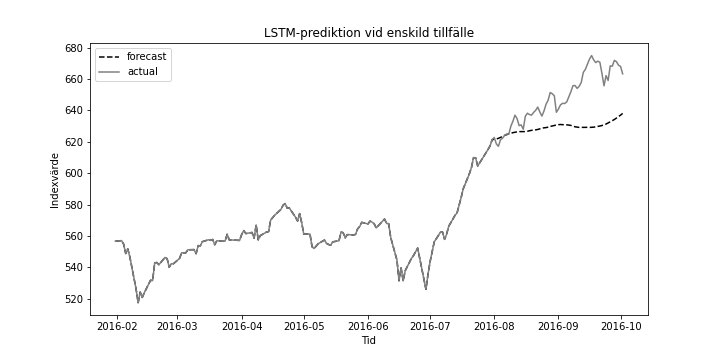
\includegraphics[width=\linewidth]{lstm_pred.png}
\centering
\end{figure}
Notera att LSTM inte har konfidensintervall.

\begin{figure}[H]
\caption{ARMA-GARCH-prediktioner vid enskild tidpunkt}
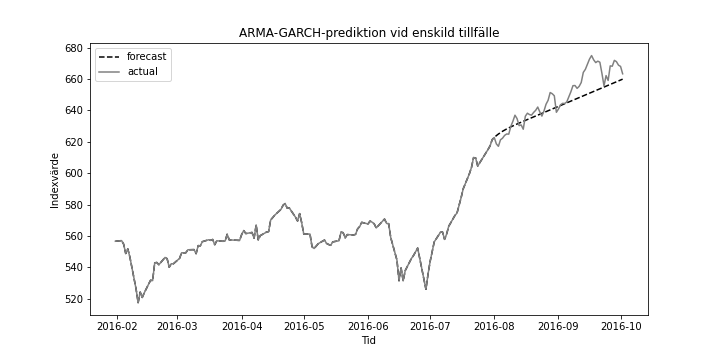
\includegraphics[width=\linewidth]{arma_garch_pred.png}
\centering
\end{figure}

\begin{figure}[H]
\caption{ARMA-GARCH-prediktioner vid enskild tidpunkt med prediktionsintervall}
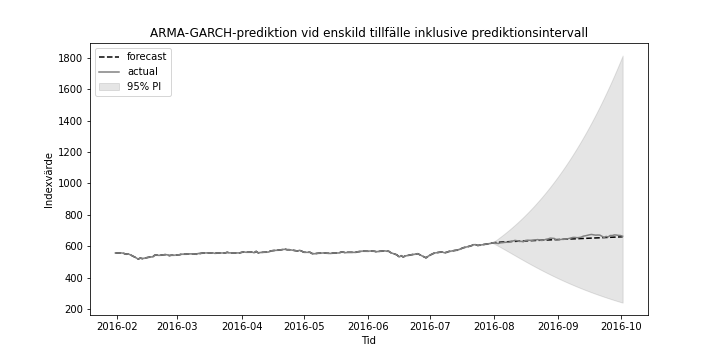
\includegraphics[width=\linewidth]{arma_garch_pred_interval.png}
\centering
\end{figure}

\newpage
\subsection{Bilaga 2 - Histogram över logaritmerad avkstning}
\begin{figure}[H]
\caption{Histogram logaritmerad avkastning}
\includegraphics[width=\linewidth]{histogram.png}
\centering
\end{figure}

\newpage
\subsection{Bilaga 3 - ADF-test}
\begin{figure}[H]
\caption{ADF-test med optimalt antal laggar}
\includegraphics[width=0.8\linewidth]{adf.png}
\centering
\end{figure}

\newpage
\subsection{Bilaga 4 - LM-test}
\begin{figure}[H]
\caption{LM-test för heteroskedasticitet}
\includegraphics[width=0.8\linewidth]{lm_test.png}
\centering
\end{figure}

\newpage
\subsection{Bilaga 5 - AIC och BIC för ett urval av modeller}
Ju lägre värde, desto bättre. ARMA(1,1)-GARCH(1,1) ger lägst resultat.
\begin{table}[H]
\caption{AIC och BIC för olika parametervärden på ARMA-GARCH}
\begin{tabular}{||lll||}
\hline
& \multicolumn{2}{l||}{Kriteria} \\
ARMA(p,q)-GARCH(p,q) & \textbf{AIC} & \textbf{BIC}\\ \hline\hline
{\textbf{(0,0)-(1,0)}} & -6.782  & -6.777 \\ \cline{2-3} 
{\textbf{(0,0)-(1,1)}} & -6.938  & -6.931 \\ \cline{2-3}
{\textbf{(0,1)-(1,1)}} & -6.951  & -6.942 \\ \cline{2-3} 
{\textbf{(1,0)-(1,1)}} & -6.954  & -6.944 \\ \cline{2-3} 
{\textbf{(1,1)-(1,1)}} & \textbf{-6.965}  & \textbf{-6.954} \\ \cline{2-3} 
{\textbf{(1,1)-(2,1)}} & -6.965  & -6.952 \\ \cline{2-3} 
{\textbf{(1,1)-(2,2)}} & -6.964  & -6.950 \\ \cline{2-3}
{\textbf{(2,1)-(2,2)}} & -6.964  & -6.948 \\ \cline{2-3} 
{\textbf{(2,2)-(2,2)}} & -6.963  & -6.946 \\ \hline
\end{tabular}
\end{table}

\newpage
\printbibliography
\end{document}